\documentclass[11pt]{article}
\usepackage{hyperref}
\usepackage{amsthm}
\usepackage{amsmath}
\usepackage{amsfonts}
\usepackage{tikz}
\usepackage{ wasysym }
\usepackage{fancyvrb}

\newtheorem{example}{Example}


\author{Group 1:  Nicholas Jacob}
\title{Homework 2 Advanced Analytics and Metaheuristics}

\begin{document}
\maketitle
%{\Large
%%Change Document name to: Graded Homework 1\_Jacob\_Nicholas
%\noindent NAME:  Nicholas Jacob\\ 
%STUDENT ID: \# 113578513\\
%HOMEWORK NUMBER: 1\\
%COURSE: DSA 5113 Advanced Analytics and Metaheuristics\\ 
%SECTION: ONLINE\\SEMESTER: Spring 2024\\
%INSTRUCTOR:  DR. Charles Nicholson\\
% SCORE:}
%
%\newpage
\begin{enumerate}
\item Grapes of Wrath
\begin{enumerate}
\item Grimes upper bound on grapes used for raisins.  We know that 25\% of the $8.4\times10^6$lb crop was ``A'' quality with the rest being ``B'' grade.  We also know that ``A grapes average 9 points per pound and ``B'' grapes average 5 points per pound.  Raisins require 8 points or higher in quality.  Here we end up with a small LP problem.  First we call $A$ the number of pounds of grade ``A'' grapes and $B$ the number of pounds of grade ``B''.  Our objective is to maximize the total pounds made into grapes:
\[
\text{maximize totalPounds: }A +B;
\]
We will have non-negative constraints on $A$ and $B$, as well as total production constraints
\[
A\leq 2 100 000\quad\text{ and }\quad B\leq 6 300 000
\]
Finally we have the quality constraint:
\[
\text{subject to qualityPoints: }9A +5B \geq 8\left(A+B\right)
\]
This one should get a small comment as we want the average number of points to be greater than 8 for our raisins.  We code this into our AMPL model and arrive at the following output.

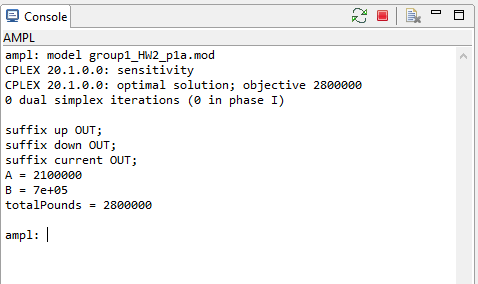
\includegraphics[width = .9\textwidth]{outputp1a.png}
\item To arrive at Bollman's assessment of the price of the grapes, it is important to consider the quality of the inputs.  We see that the entire lot was purchased for \$0.28 per pound but some of the grapes are clearly more valuable.  With the 25\% breakdown of type ``A'' to ``B'' we must account for that.  Moreover we must use the ratings to arrive at the appropriate value per pound of each type, ``A'' is rated 9 and ``B'' is rated 5, the higher the rating the more tha value to the company.  This creates a system of linear equations with $y$ begin price of type ``A'' and $z$ being price of ``B" in cents.  
\[
\left\{
\begin{array}{l}
2 100 000 y +6 300 000 z = 8 400 000 \times 28\\
\frac{y}{9} = \frac{z}{5}
\end{array}
\right.
\]
We solve this system with substitution and arrive at $y = 42$ and $z = 23\frac13$ prices reported are cents per pound.  Using these prices we see that jelly can be made entirely from the type ``B'' grapes and will require 19 pounds per product.  Therefore the grape cost for jelly is $19z = \$4.43\frac13$.  The analysis for the other two products is a bit more complicated.  Juice requires a 6 point average so if $a_j$ is the amount of high quality grapes and $b_j$ the amount of low quality grapes, we will need 
\[
9a_j+5b_j \geq 6(a_j+b_j)
\]
or
\[
3a \geq b.
\]
So for every 1 pound of high quality grapes, we can use at most 3 pounds of low quality grapes.  For purposes of computing the fruit cost, we will compute a minimum cost here but when the grapes are divided later, this price may change.  The computed minimum price for the juice grapes is
\[
15.5\frac{\left(y+3z\right)}{4} = \$4.34
\]
For the grapes, the minimum rating it 8 so
\[
9a_r+5b_r\geq 8(a_r+b_r)
\]
or
\[
a_r\geq 3b_r
\]
So each pound of low quality grapes we use in raisins, we must just at least 3 pound of high quality grapes.  We see then that the minimum price for the input grapes is \label{1b}
\[
6.75\frac{3y+z}4 = \$2.52.
\]
\item To formulate for AMPL, we ask for the decision variables to be the amount of each type of grape included in our raisins, jelly and juice.  We assume that the cost of the grapes is a fixed ratio based on quality scale points as outlined in \ref{1b} but not that the grape input should still be that fixed ratio when computing the price of our input grapes.  We consider overhead costs to be fixed and for the accounting department to figure out which product to allocate those costs to based on whatever they do in that department.
\end{enumerate}
\end{enumerate}



\end{document}
